\documentclass{beamer}

\usepackage{tikz}
\usepackage{pgfplots}

\usepackage{graphicx}
\usepackage{amsthm}
\usepackage{bm}
\usepackage{booktabs}       % professional-quality tables
\usepackage{standalone}
\usepackage{tikz}
\usepackage{pgfplots}
\usepackage{mathtools}
\usepackage[font=scriptsize]{caption}

\usetikzlibrary{bayesnet}

\let\ul\underline

\usepackage{dbt}

\setbeamertemplate{theorems}[numbered]

\pgfplotscreateplotcyclelist{my black white}{%
dashed, every mark/.append style={solid},mark=o\\%
dashed, every mark/.append style={solid, fill=gray},mark=star\\%
dotted, every mark/.append style={solid}, mark=o\\%
dotted, every mark/.append style={solid, fill=gray},mark=star\\%
solid, every mark/.append style={solid}, mark=*\\%
}
\pgfplotsset{compat=1.5}

% tikz definitions for plots
\newsavebox{\genericfilt}
\savebox{\genericfilt}{%
\begin{tikzpicture}[font=\small, >=stealth,yscale=0.15,xscale=0.1]
  % define normal distribution function 'normaltwo'
  \def\normaltwo{\x,{exp((-(\x)^2)/0.5)}}
  \draw[white, line width=0.25mm,domain=-1.7:1.7] plot (\normaltwo);
\end{tikzpicture}%
}
\newsavebox{\genericfiltLarge}
\savebox{\genericfiltLarge}{%
\begin{tikzpicture}[font=\small, >=stealth,yscale=0.25,xscale=0.2]
  % define normal distribution function 'normaltwo'
  \def\normaltwo{\x,{exp((-(\x)^2)/0.5)}}
  \draw[white, line width=0.25mm,domain=-1.7:1.7] plot (\normaltwo);
\end{tikzpicture}%
}


%\usetheme{Montpellier}
%\usecolortheme{owl}

%\usetheme{PaloAlto}
%\usecolortheme{beaver}

%\newtcolorbox{titlebox}{colback=background,colframe=CBBlue,coltext=gray}
\newtcolorbox{defbox}{colback=white,colframe=gray,coltext=black}

\newcommand{\Categorical}{\ensuremath{\mathcal{C}at}}
\newcommand\Beta{\ensuremath{\mathcal{B}eta}}
\newcommand\Bernoulli{\ensuremath{\mathcal{B}ern}}
\newcommand{\Dirichlet}{\ensuremath{\mathcal{D}ir}}
\newcommand{\Normal}{\ensuremath{\mathcal{N}}}
\newcommand{\Exponential}{\ensuremath{\mathcal{E}xp}}
\newcommand{\Poisson}{\ensuremath{\mathcal{P}oisson}}
\newcommand\DP{\ensuremath{\mathrm{DP}}}
\newcommand\GEM{\ensuremath{\mathrm{GEM}}}
\newcommand{\indpath}[2]{\mathbin{\mathcal{P}{\left(#1,#2\right)}}} % induced path
\newcommand{\indic}{\mathbbm{1}}
\newcommand{\diff}{\mathop{}\!\mathrm{d}}
\newcommand{\SPT}{\mathcal{T}}
\newcommand{\SPG}{\mathcal{C}}
\newcommand{\SPN}{\mathcal{S}}
\newcommand{\graph}{\mathcal{G}}
\newcommand{\ProductNode}{\mathsf{P}}
\newcommand{\ProductNodes}{\bm{\mathsf{P}}}
\newcommand{\SumNode}{\mathsf{S}}
\newcommand{\SumNodes}{\bm{\mathsf{S}}}
\newcommand{\Leaf}{\mathsf{L}}
\newcommand{\Leaves}{\bm{\mathsf{L}}}
\newcommand{\Node}{\mathsf{N}}
\newcommand{\Nodes}{\bm{\mathsf{N}}}
\newcommand{\Child}{\mathsf{C}}
\newcommand{\region}{\ensuremath{R}}
\newcommand{\partition}{\ensuremath{P}}
\newcommand{\regions}{\ensuremath{\mathbf{R}}}
\newcommand{\partitions}{\ensuremath{\mathbf{P}}}
\newcommand{\rg}{\ensuremath{\mathcal{R}}}

\newcommand{\X}{\mathbf{X}}
\newcommand{\data}{\mathcal{X}}
%\newcommand{\x}{\mathbf{x}}
\newcommand{\xn}{\mathbf{x}_{n}}
\newcommand{\xnd}{x_{n,d}}
\newcommand{\xd}{\mathbf{x}_{\cdot,d}}
\newcommand{\Y}{\mathbf{Y}}
\newcommand{\y}{\mathbf{y}}
\newcommand{\yd}{\mathbf{y}}
\newcommand{\ydp}{y_{d,\ProductNode}}
\newcommand{\yndp}{\mathbf{y_{\not{d},\ProductNode}}}
\newcommand{\ydP}{y_{d,\partition}}
\newcommand{\yndP}{\mathbf{y_{\not{d},\partition}}}
\newcommand{\yProduct}{\mathbf{y}_{\cdot,\ProductNode}}
\newcommand{\yPartition}{\mathbf{y}_{\cdot,\partition}}
\newcommand{\Z}{\mathbf{Z}}
\newcommand{\z}{\ensuremath{\mathbf{z}}}
\newcommand{\zn}{\ensuremath{\mathbf{z}_n}}
\newcommand{\zs}{\ensuremath{z_\SumNode}}
\newcommand{\zsn}{\ensuremath{z_{\SumNode,n}}}
\newcommand{\tld}{\ensuremath{\theta_{d,\Leaf}}}


\newcommand{\ks}{\mathbf{k}}
\newcommand{\Root}{\ensuremath{\mathbf{root}}}
\newcommand{\ch}{\ensuremath{\mathbf{ch}}}
\newcommand{\anc}{\ensuremath{\mathbf{anc}}}
\newcommand{\leaf}[1]{\mathbin{\mathbf{leaf}(#1)}} % leaf function
\newcommand{\leafs}[1]{\mathbin{\mathbf{leafs}(#1)}} % leaf function
\newcommand{\w}{w}
\newcommand{\vp}{\mathbf{v}}
\newcommand{\vps}{\mathbf{v}}
%\newcommand{\ws}{\mathbf{w}_{\SumNode}}
\newcommand{\wsc}{w_{\SumNode,\Child}}
\newcommand{\tp}{\mathbf{\theta}}
\newcommand{\val}{\ensuremath{\mathbf{val}}}
\newcommand{\scope}{\psi}
\newcommand{\cond}[2]{\mathbin{\left. #1\nonscript\;\middle|\nonscript\; #2 \right.}}
\newcommand{\cbar}{\,|\,}

\newcommand{\xnew}{\mathbf{x}^{*}}

\newcommand{\argmin}{\arg\!\min} % arg min
\newcommand{\argmax}{\arg\!\max} % arg max

\DeclareMathOperator*{\f}{\SPN(\xn \,|\, \phi)}
\DeclareMathOperator*{\fz}{\SPN(\bm \ast \,|\, \phi)}
\DeclareMathOperator*{\fy}{\SPN(\xn, \lambda_n \,|\, \phi)}
\DeclareMathOperator*{\fzy}{\SPN(\bm \ast, \lambda_n \,|\, \phi)}
\newcommand{\wa}{\w^{[0]}_{\gamma}}
\newcommand{\wb}{\w^{[1]}_{k}}
\newcommand{\wt}{\w^{(t)}_{k}}
\newcommand{\wjt}{\w^{(t)}_{j}}
\newcommand{\wjtt}{\w^{(t+1)}_{j}}
\newcommand{\wtt}{\w^{(t+1)}_{k}}
\newcommand{\wat}{\w^{[0](t)}_{\gamma}}
\newcommand{\wbt}{\w^{[1](t)}_{k}}
\newcommand{\wjbt}{\w^{[1](t)}_{j}}
\newcommand{\watt}{\w^{[0](t+1)}_{\gamma}}
\newcommand{\wbtt}{\w^{[1](t+1)}_{k}}


\AtBeginSection{\frame{\sectionpage}}
\AtBeginSubsection{\frame{\subsectionpage}}


\title{Bayesian Learning of Sum-Product Networks}
\author{\textcolor{CBPurple}{Martin Trapp\inst{1,2}} \and  R. Peharz\inst{3} \and H. Ge\inst{3} \\ F.~Pernkopf\inst{1} \and Z.~Ghahramani\inst{4,3}}
\institute{\inst{1} Graz University of Technology, %
                      \inst{2} OFAI \and
                      \inst{3} University of Cambridge, 
                      \inst{4} Uber AI}
\date{\today}


\usepackage{subfig}

\makeatletter
\let\@@magyar@captionfix\relax
\makeatother

\begin{document}

\frame{\titlepage}

\frame{
\begin{itemize}
  \item Sum-product networks (SPNs) [Poon2011] are flexible density estimators and have received significant attention due to their attractive inference properties.
  \item While parameter learning in SPNs is well developed, most structure learners are somewhat adhoc and based on intuition rather than a clear learning principle.
  \pause
  \item We introduce a well-principled Bayesian framework for SPN structure learning by decomposing the problem into:
  \begin{enumerate}
    \item laying out a computational graph, and
     \item learning the so-called scope function over the graph.
   \end{enumerate}
   \pause 
  \item We propose a natural parametrisation for an important and widely used special case of SPNs, incorporate the parameters into a Bayesian model, and perform posterior inference over structure and parameters jointly.
\end{itemize}
}

\section{Sum-Product Networks}

\frame{
\begin{center}What is a Sum-Product Network?\end{center}
\begin{itemize}
  \item Let $\X = \{X_1, \dots, X_D\}$ be set of D random variables, for which $N$ i.i.d. samples are available. 
  \item An SPN is a distribution over $\X$ defined as a 4-tuple $\SPN = (\graph, \scope, \w, \textcolor{CBOrange}{\theta})$.
  \begin{itemize}
    \pause
    \item $\graph$ is a computational graph.
    \pause
    \item $\scope$ is a so-called scope function.
    \pause
    \item $\w$ denotes the set of sum-weights and $\textcolor{CBOrange}{\theta}$ the set of leaf node parameters. 
  \end{itemize}
  \pause
  \item \textcolor{gray}{Note: This definition is conceptually different to the classic definition of SPNs as it disentangles the definition of the SPNs structure into a computational graph, which has only few requirements, and a scope function, which ensures completeness and decomposability.} 
\end{itemize}
}

\frame{
\begin{center}Computational Graph $\graph$\end{center}
\begin{itemize}
  \item Is a connected directed acyclic graph (DAG), containing three types of nodes: sums ($\SumNode$), products ($\ProductNode$) and leaves ($\Leaf$).
  \item Only encodes the topological layout of the nodes, while the effective SPN structure is encoded via the scope function $\scope$.
\end{itemize}
\pause
\begin{figure}
  \includestandalone[width=0.8\textwidth]{computation_graph}
  \caption{Example of a tree-shaped computational graph with two layers.}
\end{figure}
}

\frame{
\begin{center}Scope Function $\scope$\end{center}
\begin{itemize}
  \item Let $\Nodes$ denote the set of all nodes.
  \item $\scope$ a function $\scope \colon \Nodes \mapsto 2^\X$ assigning each node in the graph a sub-set of X ($2^\X$ denotes the power set of $\X$).
\end{itemize}
\pause
It has the following properties: 
\begin{defbox}
\begin{enumerate}
\item If $\Node$ is the root node, then $\scope(\Node) = \X$.
\item If $\Node$ is a sum or product, then $\scope(\Node) = \bigcup_{\Node' \in \ch(\Node)} \scope(\Node')$.
\item For each $\SumNode \in \SumNodes$ we have $\forall \Node, \Node' \in \ch(\SumNode)\colon \scope(\Node) = \scope(\Node')$ (\emph{completeness}).
\item For each $\ProductNode \in \ProductNodes$ we have $\forall \Node, \Node' \in \ch(\ProductNode)\colon \scope(\Node) \cap \scope(\Node') = \emptyset$ (\emph{decomposability}).
\end{enumerate}
\end{defbox}
\pause
Note: Completeness and decomposability are necessary for any SPN to be a well-defined probability distribution and to allow exact inference in linear time (in the model size).
}

\frame{
\begin{center}Example SPN $\SPN = (\graph, \scope, \w, \textcolor{CBOrange}{\theta})$\end{center}
\begin{figure}
     \centering{
        \includestandalone[width=0.7\textwidth]{computation_graph}
      }
\end{figure}
\centering $\;\;\downarrow{\;\text{Apply scope function }\scope\text{ on }\graph \;\;\;\;\;}$ 
\begin{figure}
  \centering{
    \includestandalone[width=0.7\textwidth]{SPN}
    }
\end{figure}
}

\section{Bayesian Learning of Sum-Product~Networks}

\frame{
\begin{center}Bayesian Parameter Learning\end{center}
  \begin{itemize}
    \item The key insight for Bayesian parameter learning [Zhao2016, Rashwan2016, Vergari2019] is that sum nodes can be interpreted as latent variables $Z_\SumNode$, clustering data instances.
  \end{itemize}
  \pause
  \begin{equation}
    \begin{aligned}
      \SPN(\x) &= \sum_\z \prod_{\SumNode \in \SumNodes} \w_{\SumNode, \zs} \, \prod_{\Leaf \in T(\z)} L(\x_\Leaf)  \\ &= \sum_{\SPT} \prod_{(\SumNode, \Node) \in \SPT} \w_{\SumNode, \Node} \, \prod_{\Leaf \in \SPT} \Leaf(\x_\Leaf) 
\underbrace{
\left( \sum_{\bar{\z}} \prod_{\SumNode \in \bar{\SumNodes}_\SPT} \w_{\SumNode, \bar{\zs}} \right)
}_{=1}
\end{aligned}
\end{equation} 
\pause
\begin{itemize}
  \item $\SPT$ is a so-called induced tree [Zhao2016] which is a sub-tree in $\SPN$ such that the root of $\SPN$ is the root of $\SPT$, each $\SumNode \in \SPT$ has only one child and each $\ProductNode \in \SPT$ has the same children as in $\SPN$.
  \item $T(\z)$ is a surjective (not injective) function that assigns to each value $\z$ the induced tree $\SPT$ determined by $\z$.
 \end{itemize}
}

\frame{
\begin{center}Bayesian Parameter Learning (cont.)\end{center}
  \begin{itemize}
    \item It is now conceptually straightforward to extend an SPN to a Bayesian setting, by equipping the sum-weights and leaf-parameters with suitable priors.
  \end{itemize}
  \pause
  Generative model for Bayesian parameter learning:
  \begin{equation}
\begin{aligned}
  \cond{\w_\SumNode}{\alpha} &\sim \Dirichlet(\w_\SumNode \cbar \alpha) \;\; \forall \SumNode \, ,
  &  \cond{\zsn}{\w_\SumNode} &\sim \Categorical(\zsn \cbar \w_\SumNode) \;\; \forall \SumNode \, \forall n,   \\ 
  \cond{\textcolor{CBOrange}{\theta}_\Leaf}{\gamma} &\sim p(\textcolor{CBOrange}{\theta}_\Leaf \cbar \gamma) \;\; \forall \Leaf \, ,   & 
  \cond{\x_n}{\z_n, \textcolor{CBOrange}{\theta}} &\sim \prod_{\Leaf \in T(\z_n)} \Leaf(\x_{\Leaf,n} \cbar \textcolor{CBOrange}{\theta}_\Leaf) \;\;  \forall n. 
\end{aligned} 
\end{equation}
}

\frame{
\begin{center}Bayesian Structure \& Parameter Learning\end{center}
  \begin{itemize}
    \item We introduce Bayesian learning of SPNs by considering the case in which $\graph$ is a tree-shaped region graph.
    \pause
    \item A region graph $\rg$ can be understood as a vectorised representation of SPNs and is a connected DAG containing two types of nodes: regions ($\region \in \regions$) and partitions ($\partition \in \partitions$).
  \end{itemize}
  \begin{figure}
  \centering
  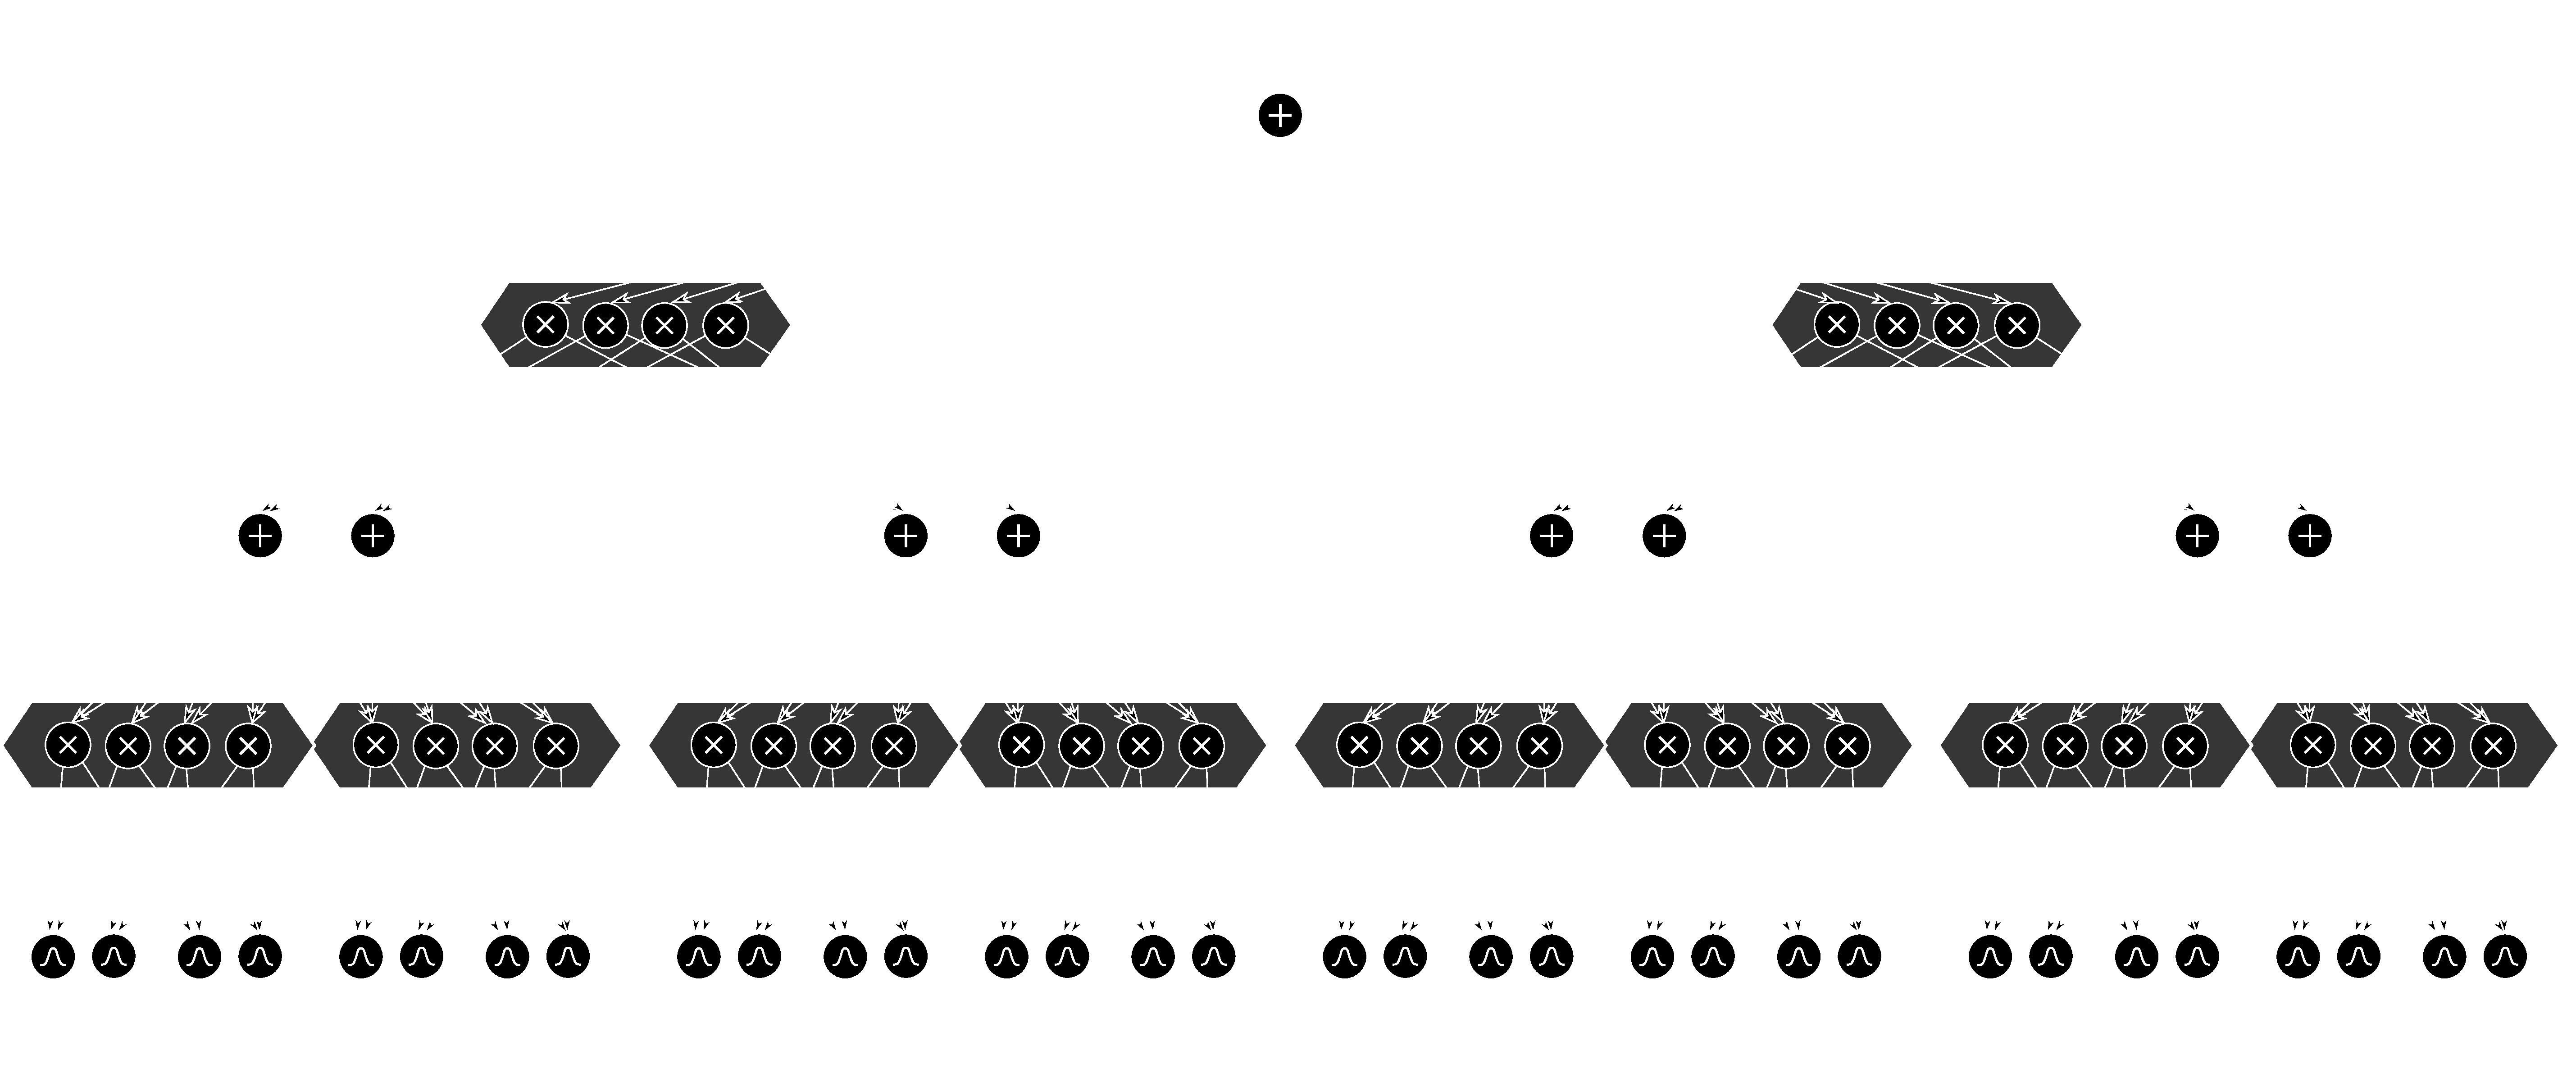
\includegraphics[width=\linewidth]{region-graph}
  \caption{Example region-graph. Based on the illustration by [Peharz2019].}
\end{figure}
}

\frame{
\begin{center}Bayesian Structure \& Parameter Learning (cont.)\end{center}
  \begin{itemize}
    \item For each data dimension d we introduce a discrete latent variable $\textcolor{CBRed}{Y}_{\partition,d}$.
    \pause
    \item The latent variable represents a decision to assign dimension $d$ to a particular child, given that all partitions above decided to assign $d$ onto the (unique) path leading to the partition
    \end{itemize}
    \pause
    Generative model for joint Bayesian learning:
    \begin{equation}
\begin{aligned}
  \cond{\w_\SumNode}{\alpha} &\sim \Dirichlet(\w_\SumNode \cbar \alpha) \;\; \forall \SumNode \, ,
  &  \cond{\zsn}{\w_\SumNode} &\sim \Categorical(\zsn \cbar \w_\SumNode) \;\; \forall \SumNode \, \forall n,   \\ 
    \cond{\vp_\partition}{\beta} &\sim \Dirichlet(\vp_\partition \cbar \beta) \;\; \forall \partition \, ,
  &  \cond{\textcolor{CBRed}{y}_{\partition,d}}{\vp_\partition} &\sim \Categorical(v_{\partition,d} \cbar \vp_\partition) \;\; \forall \partition \, \forall d,   \\ 
  \cond{\textcolor{CBOrange}{\theta}_\Leaf}{\gamma} &\sim p(\textcolor{CBOrange}{\theta}_\Leaf \cbar \gamma) \;\; \forall \Leaf ,  & 
  \cond{\x_n}{\z_n, \y, \textcolor{CBOrange}{\theta}} &\sim \prod_{\Leaf \in T(\z_n)} \Leaf(\x_{\y,n} \cbar \textcolor{CBOrange}{\theta}_\Leaf) \;\;  \forall n. 
\end{aligned}
\end{equation}
$\x_{\y,n}$ denotes the evaluation of $\Leaf$ on the scope induced by $\y$.
}

\frame{
\begin{center}Posterior Inference\end{center}
  \begin{itemize}
    \item We perform Gibbs sampling alternating between i) updating parameters $\w$, $\theta$ (fixed $\y$), and ii) updating $\y$ (fixed $\w$, $\theta$) to learn Bayesian SPNs.
    \pause
    \item This approach has shown to be sufficient for most real-world dataset, but more sophisticated approaches, e.g.~particle Gibbs combined with Hamiltonian Monte Carlo sampling; variational inference or posterior bootstrap, might be a interesting future avenues for large-scale problems. 
\end{itemize}
}

\frame{
\begin{center}Experiments (discrete data)\end{center}
  \begin{table}
%\caption{\small Avg. test LLHs for Bayesian SPNs (ours), infinite mixtures (ours$^\infty$) and best-to-date (BTD).}
  \label{tab:discrete}
  \centering
  \resizebox{\columnwidth}{!}{%
\begin{tabular}{l*{6}{r}|r}
\toprule
Dataset & LearnSPN & RAT-SPN & CCCP & ID-SPN & ours & ours$^\infty$ & BTD \\
\midrule
NLTCS & $-6.11$ & $-6.01$ & $-6.03$ & $-6.02$ & $\textcolor{CBYellow}{-6.00}$ & $-6.02$ & $-5.97$\\
MSNBC & $-6.11$ & $-6.04$ & $-6.05$ & $-6.04$ & $-6.06$ & $\textcolor{CBYellow}{-6.03}$ & $-6.03$\\
KDD & $-2.18$ & $-2.13$ & $-2.13$ & $-2.13$ & $\textcolor{CBYellow}{-2.12}$ & $-2.13$ & $-2.11$\\
Plants & $-12.98$ & $-13.44$ & $-12.87$ & $\textcolor{CBYellow}{-12.54}$ & \ul{$-12.68$} & \ul{$-12.94$} & $-11.84$\\
Audio & $-40.50$ & $-39.96$ & $-40.02$ & $-39.79$ & \ul{$\textcolor{CBYellow}{-39.77}$} & \ul{$-39.79$} & $-39.39$\\
Jester & $-53.48$ & $-52.97$ & $-52.88$ & $-52.86$ & \ul{$\textcolor{CBYellow}{-52.42}$} & \ul{$-52.86$} & $-51.29$\\
Netflix & $-57.33$ & $-56.85$ & $-56.78$ & $-56.36$ & $\textcolor{CBYellow}{-56.31}$ & $-56.80$ & $-55.71$\\
Accidents & $-30.04$ & $-35.49$ & $-27.70$ & $\textcolor{CBYellow}{-26.98}$ & \ul{$-34.10$} & \ul{$-33.89$} & $-26.98$\\
Retail & $-11.04$ & $-10.91$ & $-10.92$ & $-10.85$ & $-10.83$ & $\textcolor{CBYellow}{-10.83}$ & $-10.72$\\
Pumsb-star & $-24.78$ & $-32.53$ & $-24.23$ & $\textcolor{CBYellow}{-22.41}$ & \ul{$-31.34$}& \ul{$-31.96$} & $-22.41$\\
DNA & $-82.52$ & $-97.23$ & $-84.92$ & $\textcolor{CBYellow}{-81.21}$ & $-92.95$ & $-92.84$ & $-81.07$\\
Kosarak & $-10.99$ & $-10.89$ & $-10.88$ & $\textcolor{CBYellow}{-10.60}$ & \ul{$-10.74$} & \ul{$-10.77$} & $-10.52$\\
MSWeb & $-10.25$ & $-10.12$ & $-9.97$ & $\textcolor{CBYellow}{-9.73}$ & $-9.88$ & \ul{$-9.89$} & $-9.62$\\
Book & $-35.89$ & $-34.68$ & $-35.01$ & $-34.14$ & $\textcolor{CBYellow}{-34.13}$ & $-34.34$ & $-34.14$\\
EachMovie & $-52.49$ & $-53.63$ & $-52.56$ & $-51.51$ & $-51.66$ & $\textcolor{CBYellow}{-50.94}$ & $-50.34$\\
WebKB & $-158.20$ & $-157.53$ & $-157.49$ & $\textcolor{CBYellow}{-151.84}$ & \ul{$-156.02$} & $-157.33$ & $-149.20$\\
Reuters-52 & $-85.07$ & $-87.37$ & $-84.63$ & $\textcolor{CBYellow}{-83.35}$ & $-84.31$ & $-84.44$ & $-81.87$\\
20 Newsgrp & $-155.93$ & $-152.06$ & $-153.21$ & $\textcolor{CBYellow}{-151.47}$ & $-151.99$ & $-151.95$ & $-151.02$\\
BBC & $-250.69$ & $-252.14$ & $\textcolor{CBYellow}{-248.60}$ & $-248.93$ & $-249.70$ & $-254.69$ & $-229.21$\\
AD & $-19.73$ & $-48.47$ & $-27.20$ & $\textcolor{CBYellow}{-19.05}$ & $-63.80$ & $-63.80$ & $-14.00$\\
\bottomrule
\end{tabular}
}
\end{table}
}

\frame{
\begin{center}Experiments (heterogeneous data)\end{center}
  \begin{table}
  \centering
\begin{tabular}{lrrrr}
\toprule
Dataset & MSPN & ABDA & ours & ours$^\infty$\\
\midrule
Abalone & $\textcolor{CBYellow}{9.73}$ & $2.22$ & $3.92$ & $3.99$\\
Adult & $-44.07$ & $-5.91$ & $\textcolor{CBYellow}{-4.62}$ & $-4.68$ \\
Australian & $-36.14$ & $\textcolor{CBYellow}{-16.44}$ & $-21.51$ & $-21.99$ \\
Autism & $-39.20$ & $-27.93$ & $\textcolor{CBYellow}{-0.47}$ & $-1.16$ \\
Breast & $-28.01$ & $-25.48$ & $\textcolor{CBYellow}{-25.02}$ & $-25.76$ \\
Chess & $-13.01$ & $-12.30$ & $\textcolor{CBYellow}{-11.54}$ & $-11.76$ \\
Crx & $-36.26$ & $\textcolor{CBYellow}{-12.82}$ & $-19.38$ & $-19.62$ \\
Dermatology & $-27.71$ & $-24.98$ & $\textcolor{CBYellow}{-23.95}$ & $-24.33$ \\
Diabetes & $-31.22$ & $\textcolor{CBYellow}{-17.48}$ & $-21.21$ & $-21.06$ \\
German & $-26.05$ & $\textcolor{CBYellow}{-25.83}$ & $-26.76$ & $-26.63$ \\
Student & $-30.18$ & $\textcolor{CBYellow}{-28.73}$ & $-29.51$ & $-29.9$ \\
Wine & $\textcolor{CBYellow}{-0.13}$ & $-10.12$ & $-8.62$ & $-8.65$\\
\bottomrule
\end{tabular}
\end{table}
}

\frame{
\begin{center}Experiments (missing data)\end{center}
\begin{figure}
  \begin{minipage}{.45\textwidth}
     \begin{tikzpicture}
\begin{axis}[
    width=5.5cm,
    height=4cm,
    xlabel={\scriptsize{\% obs. with missing values}},
    ylabel={\scriptsize{test log-likelihood}},
    %ymin=-300, ymax=-249,
    legend pos=south west,
    legend columns=2,
    legend style={font=\tiny},
    legend image post style={scale=0.5},
    legend style={fill=white, fill opacity=0.6, draw opacity=1,text opacity =1},
    label style={font=\tiny},
    tick label style={font=\tiny},
    ymajorgrids=true,
    grid style=dashed,
    cycle list name=my black white
]

\addplot coordinates {
    (20, -53.551654150378006)
    (40, -54.421205612626615)
    (60, -55.51437111821264)
    (80, -57.29533673640321)
    };
\addlegendentry{LearnSPN}

\addplot coordinates {
    (20, -52.9306308300396)
    (40, -53.669159658525054)
    (60, -53.804286870223166)
    (80, -55.06448194755978)
    };
\addlegendentry{LearnSPN$^\star$}

\addplot coordinates {
    (20, -52.332443930626056)
    (40, -52.24919890693739)
    (60, -53.824333727580374)
    (80, -55.41192445685279)
    };
\addlegendentry{ID-SPN}

\addplot coordinates {
    (20, -51.71630289170897)
    (40, -52.4355408358714)
    (60, -52.30368237732657)
    (80, -53.173612370558374)
    };
\addlegendentry{ID-SPN$^\star$}

\addplot coordinates {
    (20, -51.784)
    (40, -51.997)
    (60, -52.415)
    (80, -52.85)
    };
\addlegendentry{BSPN}

\end{axis}
\end{tikzpicture}
\caption{EachMovie (D: 500, N: 5526)}
\end{minipage}
\begin{minipage}{.45\textwidth}
  \begin{tikzpicture}
\begin{axis}[
    width=5.5cm,
    height=4cm,
    xlabel={\scriptsize{\% obs. with missing values}},
    %ylabel={RMSE},
    %ymin=-168, ymax=-152,
    legend pos=north east,
    ymajorgrids=true,
    grid style=dashed,
    label style={font=\tiny},
    tick label style={font=\tiny},
    cycle list name=my black white,
    %log ticks with fixed point,
    %every axis plot/.append style={very thick}
]

\addplot coordinates {
    (20, -161.41130223478262)
    (40, -163.56351684466114)
    (60, -162.96930286251663)
    (80, -168.00941901059738)
    };
\addlegendentry{learnSPN}


\addplot coordinates {
    (20, -161.4285603783307)
    (40, -165.36322925292424)
    (60, -164.87160515320465)
    (80, -164.53405856701238)
    };
\addlegendentry{learnSPN$^\star$}

\addplot coordinates {
    (20, -152.1845925143198)
    (40, -154.95268171360382)
    (60, -158.58576871121716)
    (80, -165.45426630310263)
    };
\addlegendentry{ID-SPN}

\addplot coordinates {
    (20, -152.26143497732696)
    (40, -153.5671636300716)
    (60, -153.5671636300716)
    (80, -157.2684578353222)
    };
\addlegendentry{ID-SPN$^\star$}

\addplot coordinates {
    (20, -157.078)
    (40, -157.876)
    (60, -158.625)
    (80, -159.123)
    };
\addlegendentry{BSPN}
  \legend{}; % empty the legend so as not to print it
\end{axis}
\end{tikzpicture}
\caption{WebKB (D: 839, N: 3361)}
\end{minipage}
\begin{minipage}{.5\textwidth}
  \begin{tikzpicture}
\begin{axis}[
    width=5.5cm,
    height=4cm,
    xlabel={\scriptsize{\% obs. with missing values}},
    %ylabel={\footnotesize{test log-likelihood}},
    %ymin=0, ymax=1,
    legend pos=north east,
    ymajorgrids=true,
    grid style=dashed,
    label style={font=\tiny},
    tick label style={font=\tiny},
    cycle list name=my black white
]
 
\addplot coordinates {
    (20, -250.83622675798426)
    (40, -261.1124401206212)
    (60, -266.0005946312015)
    (80, -273.39617177834293)
    };
\addlegendentry{learnSPN}

\addplot coordinates {
    (20, -284.24099564475125)
    (40, -261.6701870807035)
    (60, -265.4755544697035)
    (80, -297.06332858812755)
    };
\addlegendentry{learnSPN$^\star$}

\addplot coordinates {
    (20, -250.68554855757577)
    (40, -253.81061585454546)
    (60, -261.81913693030305)
    (80, -272.27580261212125)
    };
\addlegendentry{ID-SPN}

\addplot coordinates {
    (20, -249.82204944242426)
    (40, -252.33469486666664)
    (60, -254.56216942424243)
    (80, -256.8125317606061)
    };
\addlegendentry{ID-SPN$^\star$}

\addplot coordinates {
    (20, -251.551)
    (40, -254.101)
    (60, -255.551)
    (80, -256.144)
    };
\addlegendentry{BSPN}
  \legend{}; % empty the legend so as not to print it
\end{axis}
\end{tikzpicture}
\caption{BBC (D: 1058, N: 1895)}
\end{minipage}
\end{figure}
}

\begin{frame}{}
\begin{center}Conclusion\end{center}
    \begin{itemize}
    \item Structure learning is an important topic in SPNs, and many promising directions have been proposed in recent years.
  \item However, most of these approaches are based on intuition and refrain from declaring an explicit and global principle to structure learning.
  \item In this paper, our primary motivation is to \emph{change} this practice
  \pause
  \item We phrase structure (and joint parameter) learning as Bayesian inference in a latent variable model. 
  \item In various experiments we show that this principled approach competes well with prior art and that we gain several benefits, such as \emph{automatic protection against overfitting}, \emph{robustness under missing data} and a natural extension to nonparametric formulations.
  \pause
  \item A critical insight for our approach is to decompose structure learning into: constructing a computational graph and separately learning the SPN's scope function.
  \end{itemize}
\end{frame}

\begin{frame}{}
\begin{center}References\end{center}
 \scriptsize $[$Poon2011$]$  H. Poon and P. Domingos. Sum-product networks: A new deep architecture. In Proceedings of UAI, pages 337–346, 2011.\\[1em]
  $[$Zhao2016$]$ H. Zhao, T. Adel, G. J. Gordon, and B. Amos. Collapsed variational inference for sum-product networks. In Proceedings of ICML, pages 1310–1318, 2016. \\[1em]
  $[$Rashwan2016$]$ A. Rashwan, H. Zhao, and P. Poupart. Online and distributed Bayesian moment matching for parameter learning in sum-product networks. In Proceedings of AISTATS, pages 1469–1477, 2016.\\[1em]
  $[$Vergari2019$]$ A. Vergari, A. Molina, R. Peharz, Z. Ghahramani, K. Kersting, and I. Valera. Automatic Bayesian density analysis. In Proceedings of AAAI, 2019.\\[1em]
  $[$Peharz2019$]$ R. Peharz, A. Vergari, K. Stelzner, A. Molina, X. Shao, M. Trapp, K. Kersting, and Z. Ghahramani. Random sum-product networks: A simple but effective approach to probabilistic deep learning. In Proceedings of UAI, 2019.\\[1em]
  \textcolor{CBYellow}{[Trapp2019] M. Trapp, R. Peharz, H. Ge, F. Pernkopf, and Z. Ghahramani. Bayesian Learning of Sum-Product Networks. To appear at NeurIPS, 2019.}
\end{frame}

\end{document}
  